\section{Experimental Setup}

\mypara{Simulation Environment} We use the Flightmare simulator~\cite{song2020flightmare} for training and testing our control policies. 
We implement the same high-level controller in \cite{mueller2018multicopter} to generates high-level commands at the level of body rates and collective thrust.
It is designed as a cascaded linear acceleration controller with desired acceleration mimicking a spring-mass-damper system with natural frequency 2rad/s and damping ratio 0.7. The desired acceleration is then converted to a desired total thrust and the desired thrust direction, and the body rates are computed from this as proportional to the attitude error angle, with a time constant of 0.2s.
% \marksez{The gains are a little hard to express compactly here. The rates are computed as (ignoring the nonlinear aspects) proportional to position, velocity, and angle error. I.e., the command has a "P" term, a "D" term, and a "double-D" term (as angle is like acceleration, to first order). 
% % Can perhaps describe it as follows:
% `We implement a custom high-level controller, that is designed as a cascaded linear acceleration controller (with desired acceleration mimicking a spring-mass-damper system with natural frequency 2rad/s and damping ratio 0.7. The desired acceleration is then converted to a desired total thrust, and desired thrust direction, and body rates are computed from this as proportional to the attitude error angle, with time constant 0.2s.'
% }
%
We define the task as hovering at a pre-defined location.
%
This high-level controller's inputs are the platform's state (position, rotation, angular, and linear velocities) and the goal location. 
%
The policy outputs individual motor speed commands, and we model the motors' response using a first-order system.
% We train the policy with model-free RL, using the PPO algorithm~\cite{schulman2017proximal}.
%
Each RL episode lasts for a maximum of 5s of simulated time, with early termination if the quadcopter height drops below 2cm.
%
The control frequency of the policy is $500$Hz, and the simulation step is 2ms.
%
We additionally implement an observation latency of 10ms.

\mypara{Quadcopter and Environment Randomization} All our training and testing ranges in simulation are listed in Table~\ref{tab:randomization}. Of these, $e_t$ includes mass, arm length, propeller torque to thrust ratio $\kappa$, motor constant, inertia ($\mathbb{R}^{3\times3}$), body drag coefficients ($\mathbb{R}^{3}$), maximum motor rotation and payload mass, which results in an 18 dimensional vector.
%
We randomize each of these parameters at the end of each episode. In addition, at a randomly sampled time during each episode, the parameters including mass, inertia, and the center of mass are also randomized. 
% \marksez{What does it mean to randomize at the end of an episode? Do we mean at the beginning of each episode? Isn't everything discarded at the end?}
%
The latter is used to mimic sudden variations in the quadcopter parameters due to a sudden disturbance caused by a payload or wind.



\mypara{Hardware Details} For all our real-world experiments we use two quadcopters, which differ in mass by a factor of 4.5, and in arm length by a factor of 2.9. 
The first one, which we name \emph{largequad} has a mass of 792g, a size of 16.6cm in arm length, a thrust-to-weight ratio of 3.50, a diagonal inertia matrix of [0.0047, 0.005, 0.0074]kg$\cdot$m$^2$ (as expressed in the z-up body-fixed frame), and a maximum motor speed of 943rad/s. The second one, \emph{miniquad}, has a mass of 177g, a size of 5.8cm in arm length, a thrust-to-weight ratio of 3.45, a diagonal inertia matrix of [92.7e-6, 92.7e-6, 158.57e-6]kg$\cdot$m$^2$, and a maximum motor speed of 3916rad/s.
%
A motion capture system running at $200$Hz provides estimates of the drone position and orientation, which is followed by a Kalman filter to reduce noise and estimate linear velocity.
%
An onboard rate gyroscope measures the angular rotation of the robot, which is low-pass filtered to reduce noise and remove outliers.
%
The deployed policy outputs motor speed commands, which are subsequently tracked by off-the-shelf electronic speed controllers.
%
We use as high-level a PD controller which takes as input the goal position and outputs the mass normalized collective trust and the body rates.

\mypara{Network Architecture and Training Procedure} The base policy is a 3-layer MLP with 256-dim hidden layers. This takes the drone state and the vector of intrinsics as input to produce motor speeds. The environment factor encoder is a 2-layer MLP with 128-dim hidden layers.  The policy and the value function share the same factor encoding layer. The adaptation module projects the latest 400 state-action pairs into a 128-dim representation, with the state-action history initialized with zeros. Then, a 3-layer 1-D CNN convolves the representation across time to capture its temporal correlation. The input channel number, output channel number, kernel size and stride of each CNN layer are [32, 32, 8, 4], [32, 32, 5, 1], [32, 32, 5, 1]. The flattened CNN output is linearly projected to estimate $z_t$. We train the base policy and the environment encoder using PPO~\cite{schulman2017proximal} for 100M steps. We use the reward outlined in Section~\ref{sec:method}. Policy training takes approximately 2 hours on an ordinary desktop machine with 1 GPU.
%
We finally train the adaptation module with supervised learning by rolling out the student policy. We train with the ADAM optimizer to minimize MSE loss. 
%
We run the optimization process for 10M steps, training on data collected over the last 1M steps. Training the adaptation module takes approximately 20 minutes.



\section{Results}

% \todo{I am unclear what the Thrust Err represent. Is the requested the Z acceleration?}

% \todo{Two more major changes which I believe are needed, more detailed investigation on unseen parameter performance, and more detail on the limitations of the work.}

% \todo{Paragraph breaks between the algorithms used in the experiment, the metrics used to compare the methods, and the final comparison would make the argument easier to read.}

% \begin{figure}[t]
%     \centering
%     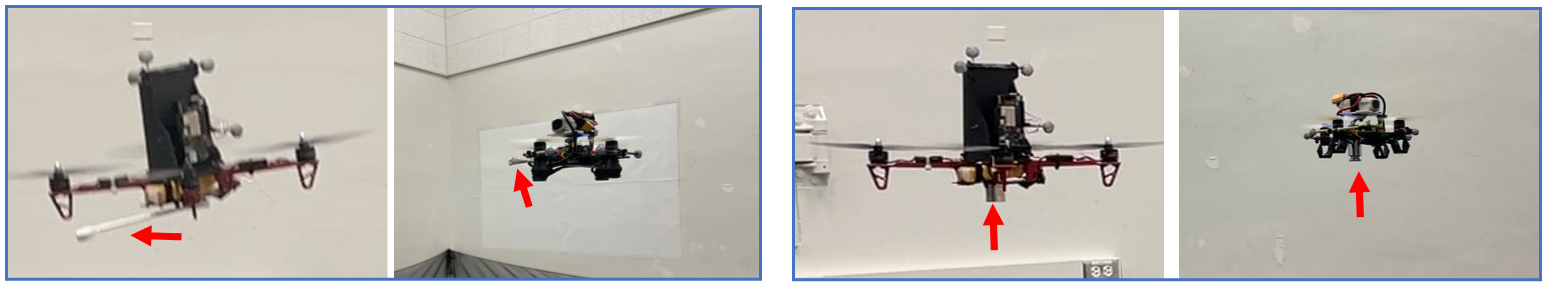
\includegraphics[width=\linewidth]{img/Disturbances_2.png}
%     \caption{\textbf{Left}: Large and small quadcopters mounted with an inertia board. For the large quadcopter, we mount a wrench of 20.5cm and 140g. For the small quadcopter, a wrench of 14.5cm and 30g. \textbf{Right}: Large and small quadcopters with a rigid payload. For the former, we add a load of 180g ($\approx 25\%$ of its weight). For the latter, we add a load of 50g, which corresponds to 35.7\% of its weight. Despite such large disturbances unknown to the control policy, our approach can always stabilize the quadcopter. Videos at~\url{https://dz298.github.io/universal-drone-controller/}}
%     \label{fig:distur}
% \end{figure}

\begin{figure}[t]
    \centering
    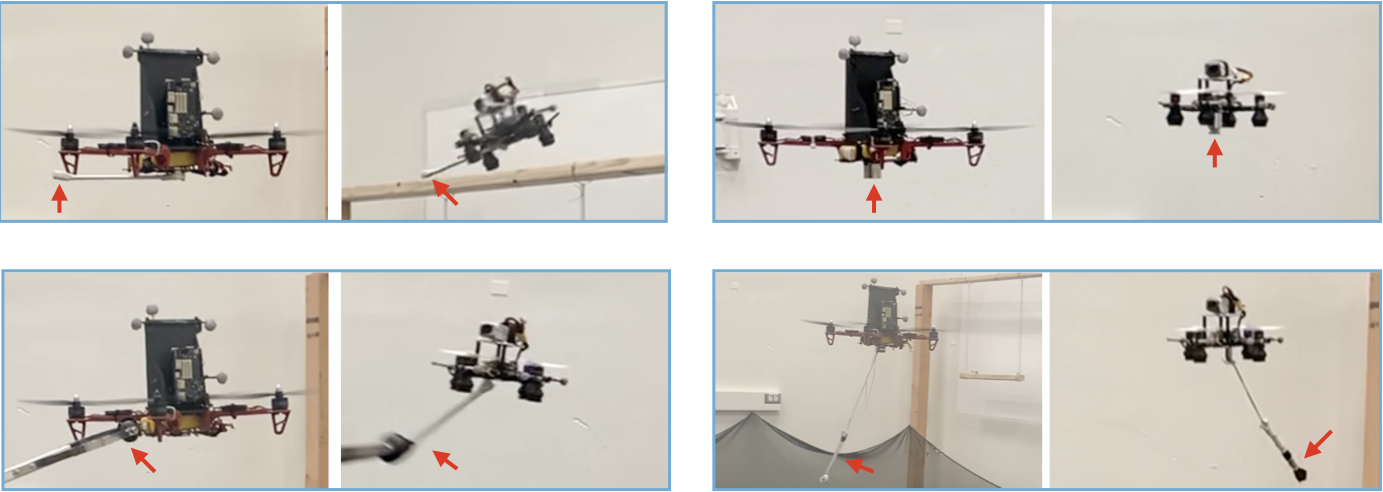
\includegraphics[width=\linewidth]{img/disturbance-include-held-out.png}
    \caption{\small \textbf{Upper Left}: Large and small quadcopters mounted with an inertia board. For the large quadcopter, we mount a wrench of 20.5cm and 140g. For the small quadcopter, a wrench of 14.5cm and 30g. \textbf{Upper Right}: Large and small quadcopters with a rigid payload. For the former, we add a load of 180g ($\approx 25\%$ of its weight). For the latter, we add a load of 50g, which corresponds to 35.7\% of its weight. \textbf{Lower Left}: Large and small quadcopters with random pushes/pulls. \textbf{Lower Right}: Large and small quadcopters with a swing payload, which is the wrench in the inertia board test. Despite such large disturbances unknown to the control policy, our approach can always stabilize the quadcopter.}
    \vspace{-3ex}
    \label{fig:distur}
\end{figure}

% Please add the following required packages to your document preamble:
% \usepackage{multirow}
% \begin{table}[t]
% \def \arraystretch{1.2}
% \centering
% % \caption{Experimental results.}
% % \label{tab:experimental_result.}
% \begin{tabular}{|l|l|l|l|l|l|}
% \hline
%  & vehicle & method & \begin{tabular}[c]{@{}l@{}}Avg. Err. \\ in height {[}m{]}\end{tabular} & \begin{tabular}[c]{@{}l@{}}Avg.  Err. \\ ang. vel. {[}rad/s{]}\end{tabular} & \begin{tabular}[c]{@{}l@{}}Avg. Err. \\ normalized thrust {[}m/s$^2${]}\end{tabular} \\ \hline
% \multirow{4}{*}{\begin{tabular}[c]{@{}l@{}}Inertial \\ board\end{tabular}} & \multirow{2}{*}{large} & PD & 0.492 & 1.347 & 1.519 \\ \cline{3-6} 
%  &  & Ours & 0.061 & 2.257 & 0.277 \\ \cline{2-6} 
%  & \multirow{2}{*}{small} & PD & 0.391 & 2.477 & 1.436 \\ \cline{3-6} 
%  &  & Ours & 0.250 & 2.351 & 0.761 \\ \hline
% \multicolumn{1}{|c|}{\multirow{4}{*}{Payload}} & \multirow{2}{*}{large} & PD & 0.617 & 0.404 & 1.744 \\ \cline{3-6} 
% \multicolumn{1}{|c|}{} &  & Ours & 0.038 & 1.251 & 0.037 \\ \cline{2-6} 
% \multicolumn{1}{|c|}{} & \multirow{2}{*}{small} & PD & 0.185 & 1.548 & 1.670 \\ \cline{3-6} 
% \multicolumn{1}{|c|}{} &  & Ours & 0.182 & 1.835 & 0.902 \\ \hline
% \end{tabular}
% \vspace{2ex}
% \caption{\label{tab:rw_results} \textbf{Real-World  Results.} We compare the performance of our controller to the PID controller which has specifically been tuned to the two quadcopters with in-flight tests. We see that our approach significantly outperforms the PD baseline in terms of average height error and tracking error on the applied thrust. The two methods perform similarly on angular velocity tracking with the PD controller sometimes outperforming our method. This is expected because our reward function favours safety over tracking performance by having a large penalty on crashing. Metrics are averaged over 5 experiments.}
% \end{table}


\begin{table}[t]
\caption{\label{tab:rw_results} \textbf{Real-World  Results:} We compare the performance of our controller to two baselines: \emph{LTF} and a PID controller. The comparison is run on three tasks for large and small quadcopters. \textbf{Free Hover}: hover at the goal position without any disturbances. \textbf{Inertia Board}: hover at the goal position under an unknown mass and inertia disturbance. \textbf{Payload}: hover at the goal position under an unknown mass disturbance.  
% The \emph{LTF} learns a robust policy to all variations seen in the training by inputting an error integration into observations, while the PID controller has specifically been tuned to the two quadcopters with in-flight tests. We see that our approach significantly outperforms the two baseline in all metrics under all disturbances, particularly in inertia board case. Our method and the PID controller perform similarly on free hovering case with the PID controller sometimes outperforming our method. This is expected because the PID controller is specifically tuned for each quadcopter. 
Metrics are averaged over 5 experiments.}
\setlength{\tabcolsep}{3pt}
\def \arraystretch{1.4}
\centering
% \caption{Experimental results.}
% \label{tab:experimental_result.}
\begin{tabular}{lllllll}
\toprule
%   \multirow{2}{*}{\textbf{External Forces}} & Success & Height  & Ang. Vel. &  Thrust \\ &Rate& Err. (m) &Err. (rad/s)  & Err. (m/s$^2$) \\%& Learning Samples\\ 
 & \multirow{2}{*}{Vehicle}& \multirow{2}{*}{Method}& Height & Ang. Vel. & Thrust& Success\\&&&Err. (m)&Err. (rad/s)&Err. (m/s$^2$)& Rate\\
\midrule
\multirow{6}{*}{\begin{tabular}[c]{@{}l@{}}\textbf{Free} \\ \textbf{Hover}\end{tabular}} & \multirow{3}{*}{small} & PID & 0.06 & 0.51 & 0.57 &  100\\ %\cline{3-6} 
&  & LTF~\cite{LTF} & 0.09 & 0.78 & 0.78 & 80 \\
 &  & Ours & 0.05 & 0.30 & 0.30 & 100 \\ \cline{2-7} 
 & \multirow{3}{*}{large} & PID & 0.01 & 0.12 & 0.28 & 100 \\ %\cline{3-6} 
 &  & LTF~\cite{LTF} & 0.03 & 1.21 & 1.86 & 80 \\
 &  & Ours & 0.03 & 0.19 & 0.36 & 100 \\ \midrule
 
 
 
\multirow{6}{*}{\begin{tabular}[c]{@{}l@{}}\textbf{Inertial} \\ \textbf{Board}\end{tabular}} & \multirow{3}{*}{small} & PID & - & - & - &  0\\ %\cline{3-6} 
&  & LTF~\cite{LTF} & - & - & - & 0 \\
 &  & Ours & 0.08 & 1.14 & 1.09 & 100 \\ \cline{2-7} 
 & \multirow{3}{*}{large} & PID & 0.31 & 0.37 & 1.46 & 100 \\ %\cline{3-6} 
 &  & LTF~\cite{LTF} & - & - & - & 0 \\
 &  & Ours & 0.08 & 0.24 & 1.35 & 100 \\ \midrule
 
 
 
\multicolumn{1}{c}{\multirow{6}{*}{\textbf{Payload}}} & \multirow{3}{*}{small} & PID & 0.40 & 1.14 & 2.20 & 80 \\ %\cline{3-6} 
&  & LTF~\cite{LTF} & 0.10 & 0.98 & 2.14 & 100 \\
\multicolumn{1}{c}{} &  & Ours & 0.05 & 0.88 & 0.51 & 100 \\ \cline{2-7} 
\multicolumn{1}{c}{} & \multirow{3}{*}{large} & PID & 0.19 & 1.14 & 1.21 & 100 \\ %\cline{3-6} 
&  & LTF~\cite{LTF} & 0.06 & 1.01 & 4.2 & 100 \\
\multicolumn{1}{c}{} &  & Ours & 0.04 & 0.34 & 1.19 & 100 \\
\bottomrule
\end{tabular}
% \vspace{2ex}
\end{table}



\subsection{Real World Deployment}

% \todo{While the evaluation of the author’s method is thorough, PID serves as a  relatively brittle real-world comparison, especially when more capable methods (e.g. L1) exists in the literature. The reviewer recognizes that comparing against existing approaches (L1, etc.) in the real world requires extensive engineering effort, but when the authors claim they are developing the first ‘universal controller,’ such effort is warranted, especially if the main application of the method is an autopilot.  The comparison against LTF is reasonable, since it is also a model free approach of drones of a wider morphology (even from the ones tested in this paper!). However, since this paper has only tested x-framed quadcopters, [6] is also a valid real world comparison as well (for the same reason as simulation results above).}

We test our approach in the physical world and compare its performance to two baselines: \emph{LTF}, which is a learning-based robust controller trained with an error integration as one of inputs, aiming to control hybrid UAVs~\cite{LTF}; and a platform-specific PID controller.
%
The PID controller has access to the platform's mass and inertia, and it has been specifically tuned to the platform with in-flight tests.
%
In contrast, our approach has no knowledge whatsoever of the physical characteristics of the system and requires no calibration or real-world fine tuning.
%
We compare the task of stabilization to a predefined set point without any disturbances (free hover), or under an unknown mass and/or inertia disturbance (Figure~\ref{fig:distur}).
%

We compare the three approaches under four metrics: (i) the average height error to the goal point, and the average tracking error of the (ii) angular velocity and (iii) mass normalized thrust of the high-level controller's commands, and the success rate.
%
We define a failure if the human operator had to intervene to avoid the quadcopter from crashing.
%
The results of these experiments are reported in table~\ref{tab:rw_results}.
%

Our approach significantly outperforms both baselines in all metrics under all disturbances. In particular, our approach achieves a 100\% success rate when asymmetric disturbances are applied to the system, while the two baselines both experience at least one total failure on either of the two platforms. 
%
The PID baseline and our approach performs similarly in free hovering experiment, with the PID controller slightly outperforming ours on \emph{largequad}.  
%
The latter difference in performance is justified, since the PID controller is specifically tuned for each quadcopter, but ours does not have knowledge of the system dynamics and hardware. 
%
% Our approach significantly outperforms the PD baseline and the LTF baseline in all metrics. in terms of success rate, average height error, and tracking error on the applied thrust.
%
% The two methods perform similarly on tracking the angular velocity commands, with the PD slightly outperforming ours in some of the tests.
%
%However, our approach significantly outperforms the PD baseline in terms of average height error and tracking error on the applied thrust.
%
% The latter difference in performance is justified by the training procedure of our controller, which favours safety to tracking performance.
%
%Indeed, we strongly penalize the agent at training time for losing height or crashing into the ground.


\subsection{Simulation Results}

% \todo{Your approach only has a 66\% success rate on the stabilization tasks. I think you should provide a more thorough discussion on the limitations and weaknesses of your approach.	What kind of conditions does your approach fail on. }

% \todo{A comparison to [6] in simulation is an absolute must. Given Belkale et al.’s good tracking error of systems with unknown dynamic parameters and quick adaptation time, the reviewer believes that this controller may also be a good universal controller candidate, even if this paper was only tested on a single drone platform.}

% \todo{When comparing against adaptive control, the argument for the author’s approach would be significantly strengthened by developing the discussion of why the removal of a ‘reference’ model and training end-to-end improves performance (what does the reference model have to do with control latency?). }

% \todo{2. Baseline selections As mentioned in Related work B -- "Learning-Based Adaptive Control", the proposed method is closely related to the other learning-based controllers, such as meta-learning approaches. Nevertheless, the experimental results are not compared with the learning-based baselines. }

% \begin{table*}[t]
% \begin{center}
% \begin{tabular*}{0.95\textwidth}{@{}lcccc@{}}
% \toprule
%   & Success Rate & Avg. Err.  & Avg.  Err. &  Avg. Err. \\ && in height [m] &ang. vel. [rad/s]  & normalized thrust \\%& Learning Samples\\ 
% \midrule
%  Robust~\cite{peng2018sim,tobin2017domain} & 4\%& 18.50 & 6.06 & 15.15 \\ 
%  SysID~\cite{SysID} & 54\%& 0.33 & 1.88 & 2.43\\
%  Ours & 64\% & 0.24 & 1.76 & 2.84 \\
% \bottomrule
% \end{tabular*}
% \caption{\label{tab:sim-metrics} \textbf{Simulation Testing Results:} We compare our method which uses adaptation in the extrinsics space, to two baselines: \emph{Robust} and \emph{SysID}. The \emph{Robust} learns a single conservative flying method for all the variations seen during training, while the \emph{SysID} baseline tries to predict the exact environment parameters which is both not difficult and not necessary to solve the task. We observe that our method which is adaptive and estimates a low dimensional extrinsics out performs both the baselines on the success rate and the average height tracking error. Because of the higher success rate, our method has to solve additional scenarios which are potentially more challenging, which explains the lower tracking error on one of the metrics. Metrics are averages over 100 experiments. 
% \vspace{-3ex}
% }
% \end{center}
% \end{table*}

\begin{table}[h]
\caption{\label{tab:sim-metrics} \textbf{Simulation Testing Results:} We compare our method with four baselines on the task of stabilization: \emph{Robust}, \emph{SysID}, \emph{LTF}, and $\mathcal{L}_1$. We also list the results of our method in Phase I training, which has access to all ground-truth system parameters and can be regarded as the expert. The test ranges are defined in Table~\ref{tab:randomization}.
% The \emph{Robust} learns a single conservative flying method for all the variations seen during training; the \emph{SysID} baseline tries to predict the exact environment parameters which is both not difficult and not necessary to solve the task; the \emph{LTF} baseline learns a robust policy with an additional input of an error integration; and the $\mathcal{L}_1$ is a model-based adaptive controller which estimates and compensates for difference between the nominal and observed states. We observe that our method which is adaptive and estimates a low dimensional intrinsics outperforms all the baselines on the success rate and the average height tracking error. Our method also achieves comparable performance on the tracking of average angular velocity and normalized thrust with baselines best on these metrics. Our method's performance is most closest to the performance of the expert Phase I which has access to the ground truth system parameters. 
Metrics are averages over 100 experiments.
}
\centering
\begin{tabular*}{0.45\textwidth}{@{}lcccc@{}}
\toprule
   & Success & Height  & Ang. Vel. &  Thrust \\ &Rate& Err. (m) &Err. (rad/s)  & Err. (m/s$^2$) \\%& Learning Samples\\ 
\midrule
 Robust~\cite{peng2018sim,tobin2017domain} & 18\%& 0.44 & 1.32 & 1.93 \\ 
 SysID~\cite{SysID} & 38\%& 0.19 & 1.10 & 1.38\\
 LTF~\cite{LTF} & 59\% & 0.35 & 0.97 & 1.68 \\
 $\mathcal{L}_1$~\cite{hanover2021performance} & 59\% & 0.17 & 0.92 & 1.60 \\
 Ours & 66\% & 0.09 & 0.94 & 1.57 \\
 \midrule
 Expert (Phase I) & 69\% & 0.09 & 0.91 & 1.29 \\
\bottomrule
\end{tabular*}
% \begin{tabular}{cccccc}
% \toprule
%               & Robust & SysID & LTF     & L1   & Ours \\
%               \midrule
% success rate  & 18\%   & 38\%  & 59\% & 59\% & 66\% \\
% \midrule
% posx err      & 0.23   & 0.07  & 0.04    & 0.01 & 0.05 \\
% posy err      & 0.14   & 0.06  & 0.09    & 0.01 & 0.18 \\
% posz err      & 0.44   & 0.19  & 0.35    & 0.17 & 0.09 \\
% \midrule
% velx err      & 0.09   & 0.08  & 0.09    & 0.11 & 0.04 \\
% vely err      & 0.10   & 0.02  & 0.14    & 0.11 & 0.12 \\
% velz err      & 0.14   & 0.07  & 0.16    & 0.16 & 0.08 \\
% \midrule
% thrust err    & 1.93   & 1.38  & 1.68    & 1.60 & 1.57 \\
% ang vel z err & 1.65   & 0.89  & 0.72    & 0.21 & 0.78 \\
% ang vel x err & 1.15   & 1.35  & 1.09    & 1.28 & 0.93 \\
% ang vel y err & 1.16   & 1.06  & 1.10    & 1.25 & 1.09 \\
% \bottomrule
% \end{tabular}
\end{table}

\begin{table}[h]
\caption{\label{tab:sim-metrics-unseen-disturb} \textbf{Simulation Testing Results, Out-of-Distribution Disturbances}: We evaluate the performance of our method and all baselines on two types of disturbances unseen at training time. \textbf{External Forces}: We apply a random force of magnitude uniformly sampled between 0 and 50\% of the weight and with direction uniformly sampled on a cube. \textbf{Partially Failing Motors}: To simulate a motor losing efficiency, we multiply the output of a randomly sampled motor’s thrust force to a random number between 0 and 1. The duration of each disturbance is random between the entire length of the episode (on and off with 2\% probability at every time stamp).
}
\centering
\begin{tabular*}{0.45\textwidth}{@{}lcccc@{}}
\toprule
  \multirow{2}{*}{\textbf{External Forces}} & Success & Height  & Ang. Vel. &  Thrust \\ &Rate& Err. (m) &Err. (rad/s)  & Err. (m/s$^2$) \\%& Learning Samples\\ 
\midrule
 Robust~\cite{peng2018sim,tobin2017domain} & 5\%& 0.39 & 2.05 & 1.51 \\ 
 SysID~\cite{SysID} & 2\%& 0.22 & 1.38 & 1.23\\
 LTF~\cite{LTF} & 32\% & 0.23 & 1.53 & 0.99 \\
 $\mathcal{L}_1$~\cite{hanover2021performance} & 42\% & 0.30 & 1.46 & 1.04 \\
 Ours & 49\% & 0.09 & 1.40 & 0.85\\
 \midrule
 \multicolumn{2}{@{}l}{\textbf{Partially Failing Motors}} &&& \\
 Robust~\cite{peng2018sim,tobin2017domain} & 1\%& 0.53 & 1.94 & 1.59 \\ 
 SysID~\cite{SysID} & 14\%& 0.33 & 1.25 & 1.23\\
 LTF~\cite{LTF} & 21\% & 0.38 & 1.57 & 1.35 \\
 $\mathcal{L}_1$~\cite{hanover2021performance} & 33\% & 0.32 & 1.41 & 1.06 \\
 Ours & 38\% & 0.26 & 1.36 & 1.01\\
\bottomrule
\end{tabular*}
\end{table}

% \begin{table*}[h]
% \centering
% \begin{tabular}{lrrrrr}
% \toprule
%                 & \multicolumn{1}{l}{SysID} & \multicolumn{1}{l}{Robust} & \multicolumn{1}{l}{LTF} & \multicolumn{1}{l}{L1}   & \multicolumn{1}{l}{Ours} \\
%                 \midrule
% success rate    & 2\%                        & 5\%                         & 32\%                     & 42\%                      & 49\%    \\
% \midrule
% posx err        & 0.43                      & 0.73                       & 0.32                    & 0.91                     & 0.32                     \\
% posy err        & 0.53                      & 0.47                       & 0.30                    & 0.92                     & 0.34                     \\
% posz err        & 0.22                      & 0.39                       & 0.23                    & 0.30                     & 0.09                     \\
% \midrule
% velx err        & 0.43                      & 0.40                       & 0.31                    & 0.30                     & 0.31                     \\
% vely err        & 0.44                      & 0.45                       & 0.29                    & 0.22                     & 0.24                     \\
% velz err        & 0.08                      & 0.13                       & 0.07                    & 0.13                     & 0.05                     \\
% \midrule
% thrust err      & 1.38                      & 2.05                       & 1.53                    & 1.46                     & 1.40                     \\
% ang vel z err   & 0.92                      & 1.63                       & 0.71                    & 0.22                     & 0.69                     \\
% ang vel x err   & 1.73                      & 1.52                       & 1.13                    & 1.45                     & 0.85                     \\
% ang vel y err   & 1.05                      & 1.36                       & 1.12                    & 1.45                     & 0.99                     \\
% \bottomrule
% \end{tabular}
% \caption{\label{tab:sim-metrics-ext-force} \textbf{Simulation Results, External Forces:}  We apply a random force of magnitude uniformly sampled between 0 and 50\% of the weight and with direction uniformly sampled on a cube. The duration is random between the entire length of the episode (on and off with 2\% probability at every time stamp).
% \vspace{-3ex}}
% \end{table*}


% \begin{table*}[h]
% \centering
% \begin{tabular}{lrrrrr}
% \toprule
%               & \multicolumn{1}{l}{Robust} & \multicolumn{1}{l}{SysID} & \multicolumn{1}{l}{LTF} & \multicolumn{1}{l}{L1} & \multicolumn{1}{l}{Ours} \\
%               \midrule
% success rate  & 1\%                        & 14\%                      & 21\%                    & 33\%                   & 38\%                     \\
% \midrule
% posx err      & 0.39                       & 0.16                      & 0.44                    & 0.10                   & 0.15                     \\
% posy err      & 0.32                       & 0.13                      & 0.20                    & 0.10                   & 0.13                     \\
% posz err      & 0.53                       & 0.33                      & 0.38                    & 0.32                   & 0.26                     \\
% \midrule
% velx err      & 0.44                       & 0.45                      & 0.53                    & 0.20                   & 0.22                     \\
% vely err      & 0.36                       & 0.19                      & 0.20                    & 0.19                   & 0.16                     \\
% velz err      & 0.61                       & 0.85                      & 1.14                    & 0.79                   & 0.90                     \\
% \midrule
% thrust err    & 1.94                       & 1.25                      & 1.57                    & 1.41                   & 1.36                     \\
% ang vel z err & 1.62                       & 0.91                      & 0.81                    & 0.23                   & 0.63               \\
% ang vel x err & 1.53                       & 1.53                      & 1.62                    & 1.48                   & 1.13                     \\
% ang vel y err & 1.63                       & 1.26                      & 1.63                    & 1.47                   & 1.26                     \\
% \bottomrule
% \end{tabular}
% \caption{\label{tab:sim-metrics-partial-motor-fail} \textbf{Simulation Results, Partially Failing Motors:}  To simulate a motor losing efficiency, we multiply the output of a randomly sampled motor’s thrust force to a random number between 0 and 1. 
% \vspace{-3ex}}
% \end{table*}



Finally, we compare our approach with a set of baselines in the simulation.
%
We select four baselines from prior work: \emph{Robust}, which consists of a policy trained without access to environment factors or body parameters~\cite{tobin2017domain, peng2018sim}; \emph{SysID}, which directly predicts the ground-truth parameters $e_t$~\cite{SysID} instead of the low-dimensional intrinsics vector; \emph{LTF}, which essentially is a robust policy with an error integration as additional inputs~\cite{LTF}; and $\mathcal{L}_1$, a model-based adaptive controller which estimates and compensates the difference between the nominal and observed states to achieve adaptive control~\cite{cao2008design,hovakimyan2010l1,hanover2021performance}. 
%
We keep the same architecture and hyperparameters as ours for all learning-based baselines. 
%
% We contacted the author of a state-of-the-art $\mathcal{L}_1$ adaptive controller ~\cite{hanover2021performance} to ensure the correctness of our implementation.\daisy{not a fan of this sentence, will remove}
%
Similarly to real-world experiments, we evaluate on the task of stabilization. The testing ranges are listed in Table~\ref{tab:randomization}. We rank the methods according to the success rate, the average height error, and the tracking performance.
%
At the beginning of each experiment, the quadcopter is spawned with a random orientation, a random position in x-y of [-1,1] and [0.5, 2.5] in z, and a random velocity on each axis of [-1,1].
%
The experiment is considered successful if the end height of the quadcopter is within 0.3m from the goal height.
%
The results of these experiments are reported in Table~\ref{tab:sim-metrics}. 
%

Given the very large amount of quadcopter variations, the \emph{Robust} baseline trained without access to environment parameters has the lowest success rate and largest tracking error. This is because it is forced to learn a single conservative controller which can fly all quadcopters under varying disturbances.
%
Indeed, it either crashes to the ground or flies outside the flying region.
%
The baseline \emph{LTF} is \emph{Robust} with an additional observation of error integration. This additional input helps it achieve higher success rate. However, similar to the \emph{Robust} baseline, \emph{LTF} fails in tracking the goal states. 
%
On the contrary, with estimation of the environment parameters, the flight performance strongly increases.
%
\begin{figure}[t]
    \centering
    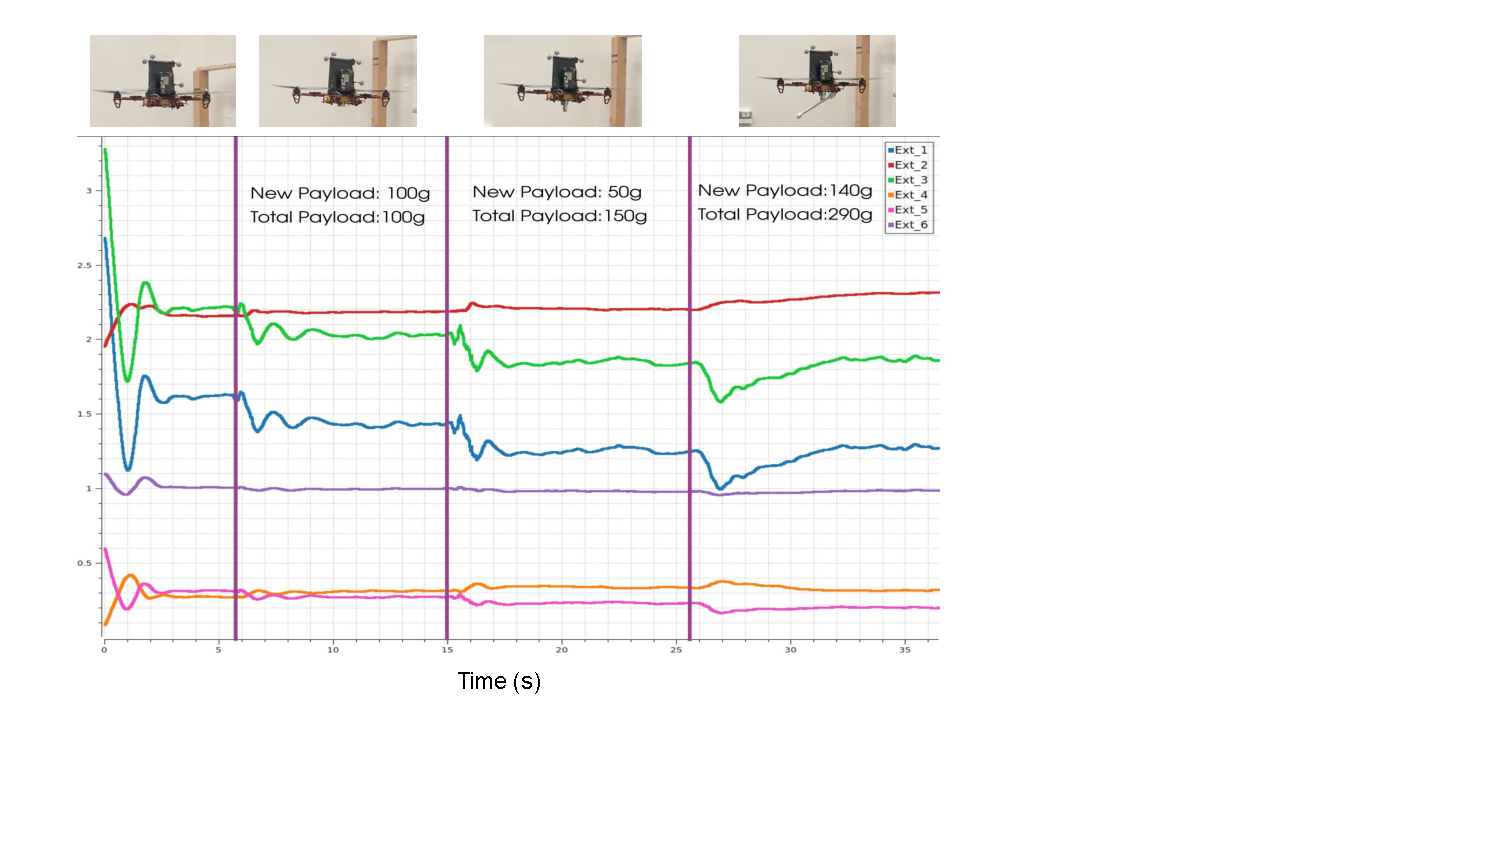
\includegraphics[width=\columnwidth]{img/extrinsics_plot_timescale.pdf}
    \caption{\small We analyze the change in behaviour of our policy as we incrementally add total 290g payloads to our \emph{largequad}. We plot all 6 components of the intrinsics vector $\hat{z_t}$ predicted by the adaptation module. We see that changes in intrinsics are strongly correlated with disturbances applied to the quadcopter, indicating that the added payloads have been detected by the adaptation module. When the payload is added, the quadcopter first sinks and then recovers to the normal motion. The plotted components of the intrinsics vector change in response to the disturbance, from which we know the adaptation period takes around 2s.}
    \label{fig:intrinsics_analysis}
\end{figure}
%
Still, explicitly regressing the environment vector $e_t$, instead of its low-dimensional representation $z_t$, yields the success rate since it is trying to solve a harder estimation problem which is not necessary to solve the task at hand.
%
Since the tracking errors are computed only for successful runs, the \emph{SysID} baseline achieves a slightly lower tracking error in one of the metrics.
%
$\mathcal{L}_1$ is the baseline with the strongest performance in our simulation experiments. However, its strong performance relies on the explicit knowledge of a reference model which we choose as the median value of all parameters in the testing range in Table~\ref{tab:randomization}, while our method with other baselines has no prior knowledge of the model. 
%
The performance gap between our method and $\mathcal{L}_1$ shows that the adaptive control across platforms is hard to achieve by estimating and compensating large variance from a reference model. 
%
$\mathcal{L}_1$ is not implemented in our real-world experiments as a baseline because it is highly sensitive to latency and requires significant engineering work. In contrast, our approach can handle latency very well by simulating it during training.
%

We also evaluate the task of stabilization on held-out environmental disturbances, as exemplified by random external forces and partial failure of a motor. The results of these experiments are reported in Table~\ref{tab:sim-metrics-unseen-disturb}. Our method outperforms all baselines in both out-of-distribution disturbances cases. Compared to the strongest baseline $\mathcal{L}_1$, our method has a greater success rate, and it reduces the average height error by up to 67.7\% and the average command tracking error by up to 22.4\%. 

% %
% Given the very large amount of quadcopter variations, the policy trained without access to environment parameters fails to achieve reasonable performance. This is because it is forced to learn a single conservative flying which can fly all quadcopters under varying disturbances.
% %
% Indeed, it either crashes to the ground or flies outside of the flying region.
% %
% Conversely, with access to environment parameters, the flight performance strongly increases.
% %
% Still, explicitly regressing the environment vector $e_t$, instead of its low-dimensional representation $z_t$ scarifies the success rate since it is trying to solve a harder estimation problem which is not necessary to solve the task at hand.
% %
% Since the tracking errors are computed only for successful runs, the \emph{SysID} baseline achieves a slightly lower tracking error on one of the metrics.
% %
% Having to solve additional scenarios which are potentially more challenging, our method accumulates a higher error, but still manages to keep the quadcopter from crashing.

% Our experiments show that whenever the policy  the importance of online adaptation.
% %
% We create a large 


\subsection{Adaptation Analysis}
We analyze the estimated intrinsics vector $\hat{z_t}$ for adaptation on incremental payloads. We incrementally add payloads in total of 290g to the \emph{largequad} in hovering. The quadcopter adapts successfully to payloads and stabilizes itself at the target position. 
%
We plot all components of the estimated intrinsics vector from the adaptation module during the experiment in Figure~\ref{fig:intrinsics_analysis}. 
%
We find that whenever a payload is applied, there is a change in all intrinsics components. 
%
% Then the quadcopter recovers from the disturbance and all components of the intrinsics vector converges to different values as they are before the payload is applied. 
% It shows that even after adaptation, the adaptation module still detects the existence of payloads. 
%
From the change of the plotted components of intrinsics vector in response to the disturbance, we see that it takes around 2s for our controller to detect the disturbance, estimate the intrinsics vector, adapt to the disturbance, and remain hovering at the target location. 
%
The adaptation period of our controller is much faster than that of methods with online estimation of ground truth model parameters such as~\cite{wuest2019online}, where it takes 10s to 15s in-flight to obtain an accurate model estimate.
